% A tervezés részletes leírása, a döntési lehetőségek értékelése és a választott megoldások indoklása

\chapter{Tervezés}

\section{Főbb tervezési szempontok}

A tervezésnél a fő szempontok az egyszerű kezelés és a sebesség voltak. Elsősorban a Photoshop szkript működését és hibáit szerettem volna figyelembe venni, hogy akik már tisztában vannak a használatával, azoknak ne jelentsen kihívást áttérni az új alternatívára, és hogy egy kellemesebb felhasználói élményt nyújtson. 

A szkript egy nagy előnye volt, hogy egy terminál helyett egy felhasználói felülete volt, és hogy mentés előtt is lehetett látni, hogy mit fog eredményezni a generálás. Sajnos egy rosszul megadott paraméter is azt jelentette, hogy az egész folyamatot elölről kellett kezdeni, ami egy kellemetlen felhasnzáló élményt eredményezett. 

Ugyan a szkript képes volt több különböző képet kezelni, az erre készült megoldás igencsak fapados volt: a mennyiséget a szkript egy szorzóként kezelte. Ez azt jelentette, hogy nem lehetett megadni egyesével, hogy adott képekből pontosan hány kerüljön elhelyezésre, a szorzó egységesen állította be a mennyiségeket.

Szerencsére nem volt gyakori eset, de előfordult már, hogy a szkriptbe egy új előbállítást kellett felvennünk. Sajnos ehhez bele kellett nyúlni a szkript forráskódjába, ahold ugyan voltak törekvések a folyamat megkönnyítésére, de még mindig egy kényszermegoldásnak minősül.
Egy ennél is primitívebb megoldás volt, ahogy bizonyos beállításcsoportok előbeállításának megválasztása kihatással volt más beállításcsoportokra, pl. egy matrica előbeállítás kiválasztása nem csak a matrica méretét határozta meg, hanem dokumentumszinten is megváltoztatta a képpontsűrűséget. Ezt a szkript úgy oldotta meg, hogy egy előbeállítás kiválasztásánál külön megvizsgálta a kiválasztott beállítást, és aszerint állította át a felhasználói felület többi területét. Ennek a konfigurálása a legkevésbé sem volt triviális, egy felhasználó nem tudná, hova kellene hozzáadni a feltételeket, és hogy azok milyen esetleges mellékhatásokkal járhatnak. 

\section{Paraméterek és csoportosításuk}

A feladathoz elengedhetetlen volt a mélyremenő és konfiguráció lehetősége, egy nyomtatásnál megannyi paramétert kell figyelembe vennünk. Ezeket a paramétereket célszerű volt valamilyen módon csoportosítani. A szkript eredetileg csak kétféle előbállításcsoportot kezelt: papírtekercs és cellaméret előbeállítások. Ezek reprezentációra itt is szükség volt, de a beállítások program bővíthetőségére való tekintettel több helyen is tovább bontottam.

\subsection{A dokumentum paraméterei}

A dokumentum beállításai a szkriptben a papírtekercs beállításaira hasonlítanak a leginkább. A dokumentum tulajdonságaihoz az alábbi dolgok tartoznak:

\begin{itemize}
    \item a dokumentum szélessége, avagy a papírtekercs szélessége.
    \item a dokumentum pixelsűrűsége\footnote{A pixelsűrűség az egységnyi hosszra eső pixelek száma.},
    \item a margók mérete,
    \item a segédvonalak beállításai,
    \begin{itemize}
        \item a segédvonalak léte,
        \item a segédvonalak vastagsága,
        \item a segédvonalak belógása,
    \end{itemize}
    \item az darabszám korrigálása\footnote{A darabszám korrigálása csak egyetlen forrásfájl esetén releváns.}.
\end{itemize}

Megoldható lett volna, hogy a segédvonalakat képenként lehessen állítani, de mivel ez szinte sosem merült fel, és mert legtöbbször minden képre vonatkozóan szeretnénk állítani segédvonalakat, ezért ezek a beállítások a dokumentum beállításai alá kerültek. 

\subsubsection{A nyomtató paraméterei}

Van pár paraméter, ami függ a nyomtató típusától, például a margók, a minimum illetve maximum dokumentummagasság.
A \plotter plotter képes teljes tekercsszélességben is nyomtatni, de ez kevésbé hatékony és ez a funkció nem garantált minden nyomtató esetén. Az alapértelmezett margó hasonlóképpen eszköztípusonként eltérő paraméter. Ugyan algoritmuselméleti szemponból a tekercset végtelennek tekinthetjük, a valóságban sajnos korlátokba ütközünk. Egyfelől a nyomtató maximális nyomtatási hossza (az említett plotteren ez kb. 18 méter), másfelől a hátralevő papírtekercs hossza is korlátoz minket, ezért indokolt, hogy ezeket az értékeket a felhasználó konfigurálni tudja.

Ezeket a paraméterek külön előbeállításcsoportként vannak kezelve, és főként bővíthetőségi okokból lettek különvéve.

\subsection{A képek paraméterei}

A szkripttel kapcsolatban egy gyakori panasz volt, hogy a képek paraméterei nem állíthatók egyesével. Ebből a hibából tanulva az alábbi paraméterek már képenként adhatók meg:

\begin{itemize}
    \item a mennyiség,
    \item a kép fizikai szélessége és magassága,
    \item a kép maszkja.
\end{itemize}

\subsubsection{A kép maszkja}

Képszerkesztésben egy kép maszkja egy olyan speciális réteget jelent, mely meghatározza, hogy a kép mely részei láthatók. A maszk egy szürkeárnyalatos kép, ahol a fekete pixelek kitakarják, a fehér pixelek átengedig, a szürke pixelek pedig részlegesen eresztik át a kép tartalmát az értéküktől függően. 

TODO kép

Feltételezzük, hogy a maszk és a maszkolni kívánt kép méretei megegyeznek. A szürkeárnyalatos pixelek $1$ és $0$ közötti értékeknek tekinthetők, ahol a fehér pixelek értéke a legmagasabb.
Ezek alapján, ha $k$ képet $m$ maszkkal szeretnénk maszkolni, úgy az eredmény $k'$, ahol a kép minden $i, j$ pixelének alfa csatornájanak értéke:

$$k'_\alpha(i, j) = k_\alpha(i, j) * m(i, j).$$

Kitűzők és matricák nyomtatásánál általában valamilyen kör alakú formára vágjuk fel a kinyomtatott képeket, ezért a szkriptben lehetőség volt ezeket a képeket egy kör alakú mintával maszkolni, ami így egy kör alakú képet eredményezett.

Vitatható, hogy a maszkolás mennyire tartozik a program feladatkörébe. Egyfelől vannak erre specializálódó programok, ahol előre láthatjuk a maszkolás eredményét, és még helyben korrigálni tudjuk a képet. Másfelől ez egy olyan funkció volt, melynek elhagyása egy visszalépést jelentett volna a szkripttől, és általában nem álltak rendelkezésünkre az előre maszkolt képek. 
A kör alak sokszor elősegíti a vágást, és gyakran kevesebb tintát használ fel, hiszen nem pazarlunk festéket a levágandó részekre.
Ugyan a feladat csak a papírfelesleg minimalizálását foglalja magában, de a kevesebb tinta használata kisebb nyomtatási költségekhez vezet, ami nem csak nekünk, hanem más nyomdáknak is egy előnyt jelenthet. Mindezek miatt úgy döntöttem, hogy megtartom ezt a funckionalitást.

A maszkhoz tartozó előbeállítás tartalmazza a maszk képének elérési útvonalát. Ez az előbeállítás is főként bővíthetőségi okok miatt lett különvéve.

\section{Kaszkádos előbeállítások}

A paraméterek nagyon gyakran valamilyen szabványnak vagy előre megadott értéknek felelnek meg. Ez különösen igaz a képek méretére (pl. A4-es szabvány) és a papírtekercsek szélességére. 

Ezeknek a méreteknek nem szeretnénk mindig utánajárni, és fejben tartani sem egyszerű, ezért nagy segítség, hogyha a legtöbbet használt méretekhez és konfigurációkhoz a program előbállításokat nyújt. 
Ezeket az előbeállítások fájlokból célszerű beolvasni, hogy azt egy felhasználó is szerkeszteni illetve bővíteni tudja a program újrafordítása nélkül. Ez a flexibilitás elősegíti, hogy más nyomdák is egyszerűen át tudjanak térni a program használatára, és hogy egy elkerülhetetlen jövőbeli plottercsere ne okozzon problémát és ne eredményezze a program elavulását.

Mind a négy beállításcsoporthoz tartozhatnak előbeállítások, amiket valamilyen fájlból lehet betölteni, adott séma alapján. 
Egy másik apró, de nagyon hasznosnak bizonyuló ötlet volt, hogy ne legyen kötelező minden paramétert megadni egy előbeállítás fájlban, és hogy ezekre az értékekre ne legyen hatással a beállítás betöltésének folyamata, ne vesszenek el az esetleg eddig beállított értékek, ha nem vonatkozik rá az előbeállítás. 
Ezek alapján valamilyen félig strukturált módon érdemes tárolnunk az előbeállításokat, pl. kulcs-érték formában.

Egy hasznos funckionalitás volt, hogy egy előbeállítás a betöltésekor másik beállításcsoportokra is kihatással lehetett. A funkció szkriptbeli implementációja nem volt hatékony, vinszont meg szerettem volna tartani, így egy új megközelítéssel próbáltam megoldani.
Az elképzelésem az volt, hogy adott előbeállítás fájlok magukban tartalmazhatnak más csoportokhoz tarzotó paramétereket, mint alcsoportok vagy referenciák más fájlokra. A program az előbeállítások betöltéskor megvizsgálja, hogy a fájl tartalmaz-e alcsoportokat, és ha igen, az alcsoport tartalmát továbbadja a megfelelő beállításcsoportért felelős komponensnek, ahol az alcsoport betöltésre kerül. A cél az, hogy az alcsoportok sémája megegyezzen az adott beállításcsoport sámájával, így továbbadáskor a komponensnek ne kelljen tudatában lennie, hogy alcsoportot tölt éppen be, vagy sem.

\section{Osztályarchitekúra}

A program architektúrájának tervezésekor nagy hangsúlyt kapott a teljesítmény. 

mindent csak egyszer tárolunk, mindent csak egyszer szűrünk stb.

optimalizációs megfontolások
ügyelés a bővíthetőségre

\section{A felhasználói felület}

mit akartam látni a uion, ui megfontolások
TODO ui vázlat

A tervezéshez UML diagramokat készítettem. 


A projekt a \texttt{printf} nevet kapta.

\begin{figure}[h]
    \centering
    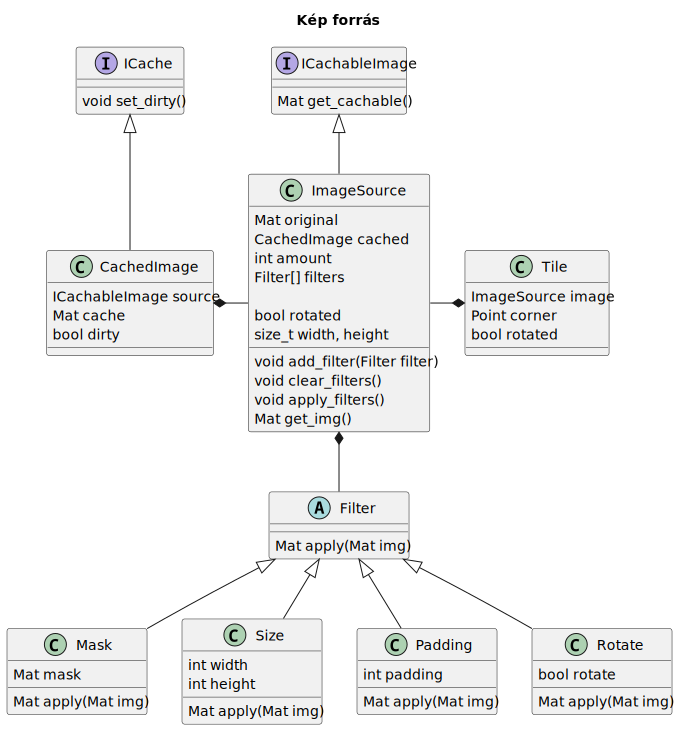
\includegraphics[width=15cm]{figures/uml/img_source.pdf}
    \label{fig:ImageSource_uml}
\end{figure}

\begin{figure}[h]
    \centering
    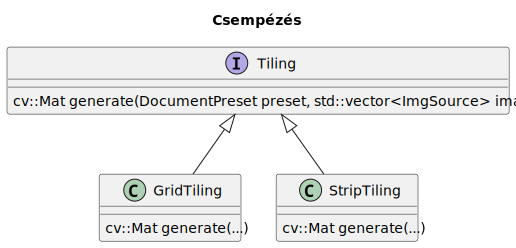
\includegraphics[width=12cm]{figures/uml/tiling.pdf}
    \label{fig:Tiling_uml}
\end{figure}

\begin{figure}[h]
    \centering
    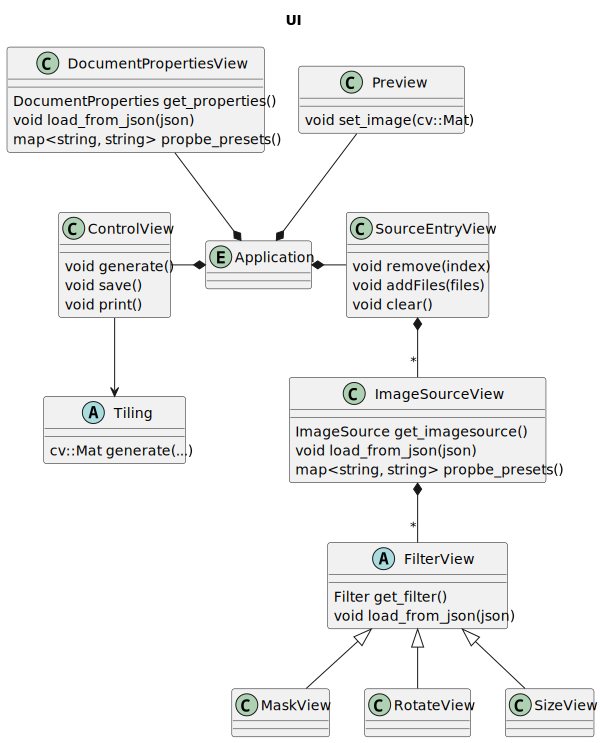
\includegraphics[width=14cm]{figures/uml/ui.pdf}
    \label{fig:UI_uml}
\end{figure}


\section{Kép betöltés, konfigurálás}

%A bemeneti képeket tartalmazó és manipuláló osztályok tervezésénél különösen nagy hangsúlyt helyeztem a teljesítményre. Az \href{fig:ImageSource_uml}{ábrán} látszik, hogy a forrásfájlokat pixelenként tároljuk, és számon tartjuk a hozzájuk tartozó filtereket. A filterek tudják transzformálni és manipulálni a képet (pl. méret, forgatás, maszk, segédvonalak). Az eredeti képet mindig megőrizzük, hogy a filterek ne legyenek destruktívak. Annak érdekében, hogy a filtereket ne kelljen minden egyes elérésnél újra számolni vezettem be egy cachet. Ha változnak a filterek, a cache piszkos lesz, és a következő elérésnél újra számolódik.

%Ennek fényében úgy döntöttünk, hogy támogatjuk mindkét megközelítést, és majd a felhasználó dönt a különböző algoritmusok között. Erre a célra szolgál egy Tiling interface, ami megkapja a képek listáját és a dokumentum tulajdonságait.

\section{A felhasználói felület}

%A legnagyobb szabadságunk a felhasználói felület kapcsán volt. Mindenképpen szerettem volna egy előnézetet, hogy még mentés előtt a felhasználó láthassa az eredményt, és azt esetleg javítani tudja a beállítások újra konfigurálásával. A kezelés lépéseinek sorrendje alapján igyekeztem kialakítani a felület többi részét. Vannak bemeneti képeink, azokat szeretnénk egyesíteni, majd kinyomtatni. Képek, egyben, nyomtatás. Ezeket balról jobbra elrendezve kapjuk meg a felület végleges tervét: balra a bemenetek és azok beállításai, középen egy előnézet, jobbra pedig a kimenet (generált dokumentum) beállításai, a generálás és az exportálás/nyomtatás gomb. A UI feladata lenne továbbá az előbeállítások betöltése és a filterek beállításainak kezelése is. A bemenetek alapján meghívódik a generálás, ami elkészíti nekünk a kívánt képet, ezt fogjuk látni az előnézeten.



